
\hypertarget{menu_search}{}
\section{Search}
\index{search menu}

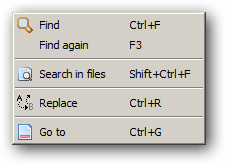
\includegraphics[scale=0.50]{./res/menu_search.png}\\

\begin{scriptsize}\begin{tabularx}{\textwidth}{>{\hsize=0.2\hsize}X>{\hsize=.8\hsize}X}\\
    \hline
    \textbf{Option} & \textbf{Description} \\
    \hline
    Find & Opens the \htmladdnormallink{Find}{\#working\_findreplace} dialog \\
    \hline
    Find again & Uses the previously entered search criteria to find the next occurrence,
    i.e, one closer to the end of the file. This option is not available if a search has not been carried out. \\
    Search in files & Opens the \htmladdnormallink{Search in files}{\#working\_searchinfiles} dialog \\
    Replace & Opens the \htmladdnormallink{Replace}{\#working\_findreplace} dialog \\
    Go to & This option produces the dialog below and allows you to move the cursor to the specified position \\
    \hline
  \end{tabularx}\end{scriptsize}
